% Revision v3, 2026-11-05. Figure 10.2.
\documentclass[border=5pt]{standalone}
\usepackage{fontspec}
\usepackage{unicode-math}
\setmainfont{Noto Sans}
\setsansfont{Noto Sans}
\newfontfamily\FigureItalic{Noto Serif}
\setmathfont{STIXTwoMath-Regular.otf}
\usepackage{tikz}
\usetikzlibrary{arrows.meta,calc,decorations.pathmorphing,decorations.markings,decorations.pathreplacing,shapes.geometric}
\definecolor{Ink}{HTML}{000000}
\definecolor{Curve}{HTML}{000000}
\definecolor{Muted}{HTML}{000000}
\tikzset{
 ax/.style={draw=Ink,line width=.72pt,-{Latex[length=2.3mm,width=1.45mm]}},
 lev/.style={draw=Ink,line width=1.50pt,line cap=butt},
 helper/.style={draw=Muted,line width=.65pt},
 bare/.style={draw=Muted,line width=.94pt,dash pattern=on 4pt off 2.5pt},
 curve/.style={draw=Curve,line width=1.85pt,line cap=round,line join=round},
 ray/.style={draw=Ink,line width=1.05pt,-{Latex[length=2.3mm,width=1.5mm]}},
 measure/.style={draw=Ink,line width=.85pt,{Latex[length=1.9mm,width=1.3mm]}-{Latex[length=1.9mm,width=1.3mm]}},
 flow/.style={draw=Ink,line width=1.05pt,postaction={decorate},decoration={markings,mark=at position .67 with {\arrow{Latex[length=2.3mm,width=1.5mm]}}}},
 link/.style={draw=Ink,line width=1.07pt},
 wave/.style={draw=Ink,line width=1.0pt,decorate,decoration={snake,amplitude=.34mm,segment length=2.7mm,pre length=1.0mm,post length=1.0mm}},
 lab/.style={text=Ink,font=\fontsize{14}{17}\selectfont,inner sep=2pt},
 small/.style={text=Ink,font=\fontsize{12.5}{15}\selectfont,inner sep=2pt},
 tag/.style={text=Ink,font=\fontsize{14}{17}\selectfont\FigureItalic\itshape,inner sep=2pt}}
\pagestyle{empty}
\begin{document}
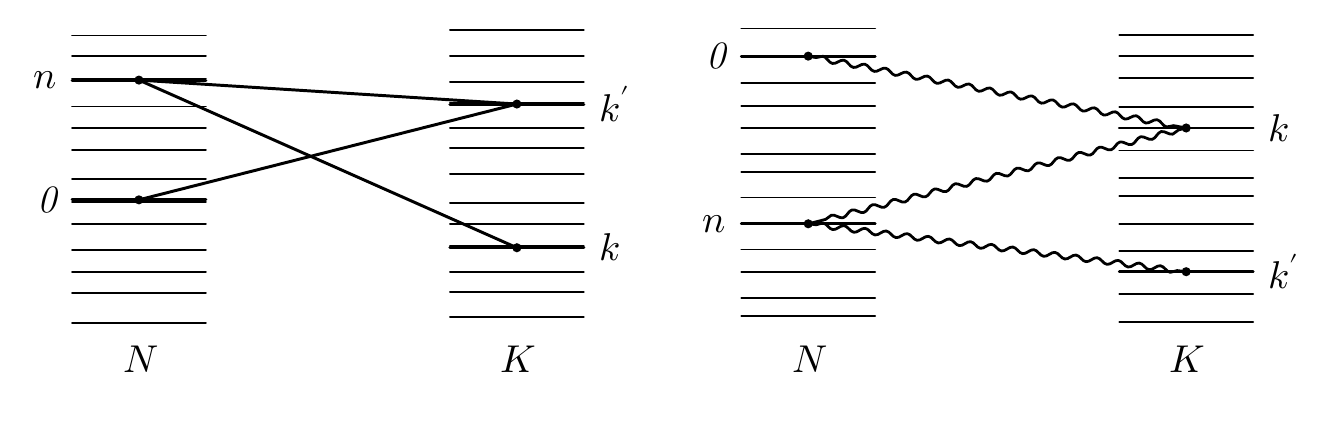
\begin{tikzpicture}[x=1cm,y=1cm,line cap=round,line join=round]
% 10.2 p.130: straight/wavy lines represent coupling factors of two amplitudes.
% Uniform row layout is diagrammatic, NOT a hypothesis of equal physical energies.
% All level strokes share one width. Every selected state belongs to the row list.

\draw[helper] (0.550000,0.509000) -- (2.250000,0.509000);
\draw[helper] (0.550000,0.883167) -- (2.250000,0.883167);
\draw[helper] (0.550000,1.158333) -- (2.250000,1.158333);
\draw[helper] (0.550000,1.431500) -- (2.250000,1.431500);
\draw[helper] (0.550000,1.766667) -- (2.250000,1.766667);
\draw[helper] (0.550000,2.047833) -- (2.250000,2.047833);
\draw[helper] (0.550000,2.334000) -- (2.250000,2.334000);
\draw[helper] (0.550000,2.708167) -- (2.250000,2.708167);
\draw[helper] (0.550000,2.983333) -- (2.250000,2.983333);
\draw[helper] (0.550000,3.256500) -- (2.250000,3.256500);
\draw[helper] (0.550000,3.610667) -- (2.250000,3.610667);
\draw[helper] (0.550000,3.895833) -- (2.250000,3.895833);
\draw[helper] (0.550000,4.159000) -- (2.250000,4.159000);
\draw[helper] (5.350000,0.579000) -- (7.050000,0.579000);
\draw[helper] (5.350000,0.900167) -- (7.050000,0.900167);
\draw[helper] (5.350000,1.158333) -- (7.050000,1.158333);
\draw[helper] (5.350000,1.481500) -- (7.050000,1.481500);
\draw[helper] (5.350000,1.766667) -- (7.050000,1.766667);
\draw[helper] (5.350000,2.029833) -- (7.050000,2.029833);
\draw[helper] (5.350000,2.404000) -- (7.050000,2.404000);
\draw[helper] (5.350000,2.725167) -- (7.050000,2.725167);
\draw[helper] (5.350000,2.983333) -- (7.050000,2.983333);
\draw[helper] (5.350000,3.306500) -- (7.050000,3.306500);
\draw[helper] (5.350000,3.568667) -- (7.050000,3.568667);
\draw[helper] (5.350000,3.895833) -- (7.050000,3.895833);
\draw[helper] (5.350000,4.229000) -- (7.050000,4.229000);
\draw[link] (0.550000,3.591667) -- (2.250000,3.591667);
\node[lab,anchor=east] at (0.430000,3.591667) {$n$};
\draw[link] (0.550000,2.070833) -- (2.250000,2.070833);
\node[lab,anchor=east] at (0.430000,2.070833) {{\FigureItalic\itshape 0}};
\draw[link] (5.350000,3.287500) -- (7.050000,3.287500);
\node[lab,anchor=west] at (7.170000,3.287500) {$k'$};
\draw[link] (5.350000,1.462500) -- (7.050000,1.462500);
\node[lab,anchor=west] at (7.170000,1.462500) {$k$};
\node[lab] at (1.400000,0.050000) {$N$};
\node[lab] at (6.200000,0.050000) {$K$};
\draw[link] (1.400000,2.070833) -- (6.200000,3.287500);
\draw[link] (6.200000,3.287500) -- (1.400000,3.591667);
\draw[link] (1.400000,3.591667) -- (6.200000,1.462500);
\fill[Ink] (1.400000,3.591667) circle (1.65pt);
\fill[Ink] (1.400000,2.070833) circle (1.65pt);
\fill[Ink] (6.200000,3.287500) circle (1.65pt);
\fill[Ink] (6.200000,1.462500) circle (1.65pt);
\node[tag] at (3.800000,-0.460000) {а};
\begin{scope}[shift={(8.50,0)}]
\draw[helper] (0.550000,0.596000) -- (2.250000,0.596000);
\draw[helper] (0.550000,0.823167) -- (2.250000,0.823167);
\draw[helper] (0.550000,1.158333) -- (2.250000,1.158333);
\draw[helper] (0.550000,1.439500) -- (2.250000,1.439500);
\draw[helper] (0.550000,1.766667) -- (2.250000,1.766667);
\draw[helper] (0.550000,2.099833) -- (2.250000,2.099833);
\draw[helper] (0.550000,2.421000) -- (2.250000,2.421000);
\draw[helper] (0.550000,2.648167) -- (2.250000,2.648167);
\draw[helper] (0.550000,2.983333) -- (2.250000,2.983333);
\draw[helper] (0.550000,3.264500) -- (2.250000,3.264500);
\draw[helper] (0.550000,3.550667) -- (2.250000,3.550667);
\draw[helper] (0.550000,3.895833) -- (2.250000,3.895833);
\draw[helper] (0.550000,4.246000) -- (2.250000,4.246000);
\draw[helper] (5.350000,0.519000) -- (7.050000,0.519000);
\draw[helper] (5.350000,0.873167) -- (7.050000,0.873167);
\draw[helper] (5.350000,1.158333) -- (7.050000,1.158333);
\draw[helper] (5.350000,1.421500) -- (7.050000,1.421500);
\draw[helper] (5.350000,1.766667) -- (7.050000,1.766667);
\draw[helper] (5.350000,2.116833) -- (7.050000,2.116833);
\draw[helper] (5.350000,2.344000) -- (7.050000,2.344000);
\draw[helper] (5.350000,2.698167) -- (7.050000,2.698167);
\draw[helper] (5.350000,2.983333) -- (7.050000,2.983333);
\draw[helper] (5.350000,3.246500) -- (7.050000,3.246500);
\draw[helper] (5.350000,3.620667) -- (7.050000,3.620667);
\draw[helper] (5.350000,3.895833) -- (7.050000,3.895833);
\draw[helper] (5.350000,4.169000) -- (7.050000,4.169000);
\draw[link] (0.550000,3.895833) -- (2.250000,3.895833);
\node[lab,anchor=east] at (0.430000,3.895833) {{\FigureItalic\itshape 0}};
\draw[link] (0.550000,1.766667) -- (2.250000,1.766667);
\node[lab,anchor=east] at (0.430000,1.766667) {$n$};
\draw[link] (5.350000,2.983333) -- (7.050000,2.983333);
\node[lab,anchor=west] at (7.170000,2.983333) {$k$};
\draw[link] (5.350000,1.158333) -- (7.050000,1.158333);
\node[lab,anchor=west] at (7.170000,1.158333) {$k'$};
\node[lab] at (1.400000,0.050000) {$N$};
\node[lab] at (6.200000,0.050000) {$K$};
\draw[wave] (1.400000,3.895833) -- (6.200000,2.983333);
\draw[wave] (6.200000,2.983333) -- (1.400000,1.766667);
\draw[wave] (1.400000,1.766667) -- (6.200000,1.158333);
\fill[Ink] (1.400000,3.895833) circle (1.65pt);
\fill[Ink] (1.400000,1.766667) circle (1.65pt);
\fill[Ink] (6.200000,2.983333) circle (1.65pt);
\fill[Ink] (6.200000,1.158333) circle (1.65pt);
\node[tag] at (3.800000,-0.460000) {б};
\end{scope}
\end{tikzpicture}

\end{document}
